\lab{Speech Recognition using CDHMMs}{Speech Recognition using CDHMMs}
\objective{Understand how speech recognition via CDHMMs works, and implement a simplified speech recognition system.}

\subsection{Continuous Density Hidden Markov Models}
Some of the most powerful applications of Hidden Markov Models, speech and voice recognition, result from allowing the observation space to be continuous instead of discrete.
These are called Continuous Density Hidden Markov Models (CDHMMs), and they have two standard formulations: Gaussian HMMs and Gaussian Mixture Model HMMs (GMMHMMs).
The former is a special case of the latter, so we will just discuss GMMHMMs in this lab.

In order to understand GMMHMMs, we need to be familiar with a particular continuous, multivariate distribution called a \emph{mixture of Gaussians}.
A mixture of Gaussians is a distribution composed of several Gaussian distributions with corresponding weights.
Such a distribution is parameterized by the number of mixture components $K$ (where each component is a Gaussian distribution), the dimension $M$ of the normal distributions involved, a collection of component weights
$\{c_1, \ldots, c_K\}$ that are nonnegative and sum to 1, and a collection of mean and covariance parameters $\{(\mu_1,\Sigma_1), \ldots, (\mu_K,\Sigma_K)\}$ for each Gaussian
component. To sample from a mixture of Gaussians, one first chooses the mixture component $i$ according to the probability weights $\{c_1,\ldots,c_K\}$, and then one
samples from the normal distribution $\mathcal{N}(\mu_k, \Sigma_k)$. The probability density function for a mixture of Gaussians is given by
\[
p(\mathbf{z}|\mathbf{\theta}) = \sum_{k=1}^K c_kN(\mathbf{z};\,\mu_k,\Sigma_k),
\]
where $N(\text{ } \cdot \text{ };\,\mu_k,\Sigma_k)$ denotes the probability density function for the normal distribution $\mathcal{N}(\mu_k, \Sigma_k)$.
See Figure \ref{fig:mixture} for the plot of such a density curve.
Note that a mixture of Gaussians with just one mixture component reduces to a simple normal distribution, and so a GMMHMM with just one mixture component
is simply a Gaussian HMM.

\begin{figure}
\centering
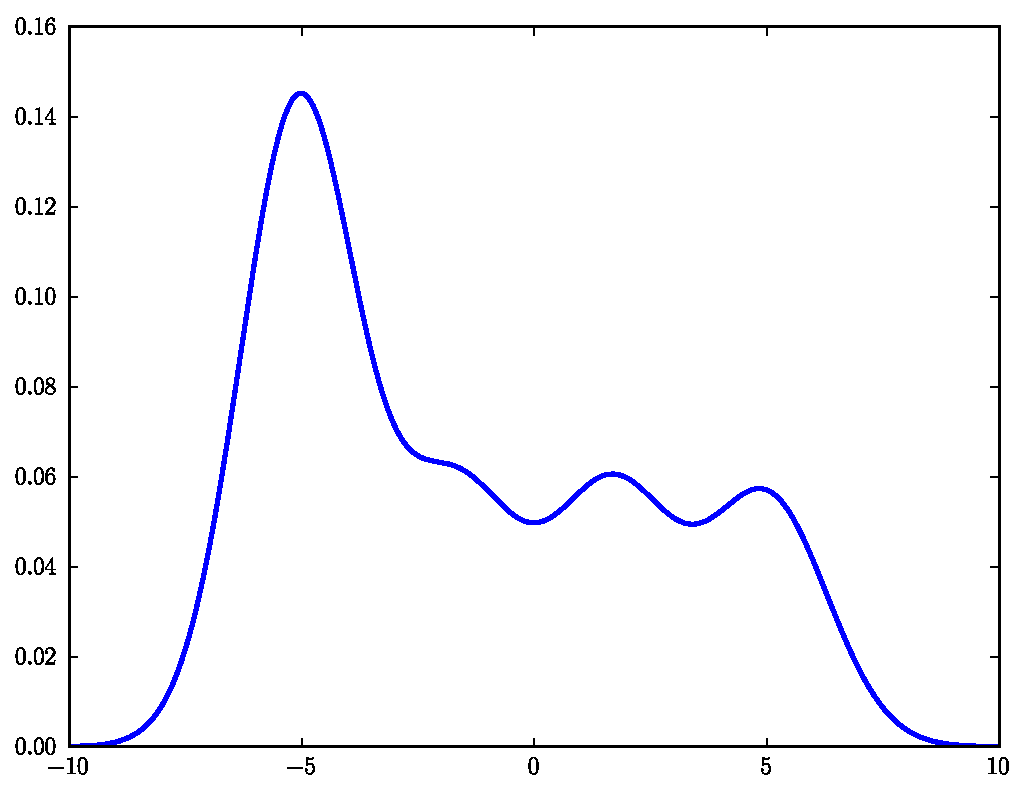
\includegraphics[width=\textwidth]{mixture}
\caption{The probability density function of a mixture of Gaussians with four components.}
\label{fig:mixture}
\end{figure}


Similar to discrete HMMs, GMMHMMs seek to model a hidden state sequence $\{X_1,\ldots, X_T\}$ and a corresponding observation sequence $\{Z_1,\ldots,Z_T\}$ where $T$ is the number of time steps or number of observations.
The major difference is that each observation $\mathbf{z}_t$ is a real-valued vector of length $M$ distributed according to a mixture of Gaussians with $K$ components.
The parameters for such a model include the initial state distribution $\pi$ and the state transition matrix $A$ (just as with discrete HMMs).
Additionally, for each state $i=1,\ldots,N$, we have component weights $\{c_{i,1},\ldots,c_{i,K}\}$, component means $\{\mu_{i,1},\ldots,\mu_{i,K}\}$, and component covariance matrices
$\{\Sigma_{i,1},\ldots,\Sigma_{i,K}\}$.

Let's define a full GMMHMM with $N=3$ states, components of dimension $M = 2$, and $K=5$ components.
\begin{lstlisting}
>>> import numpy as np

# 3x3 transition matrix 
>>> A = np.array([[.6, .3, .1], [.2, .3, .5], [.7, .1, .2]])

# 3x5 collection of component weights
>>> weights = np.array([[.5, .1, .25, .09, 0.6], [0, .4, .3, .2, .1], [.1, .3, .2, .1, .3]])

# 3x5x2 collection of component means
>>> means = np.array([np.floor(np.random.uniform(-20, 20, size = (5, 2))) for i in range(3)])

# 3x5x(2x2) collection of component covariance matrices       
>>> covars = np.array([[np.floor(np.random.uniform(1, 20))*np.eye(2) for i in range(5)] for j in range(3)])

# (3,) ndarray initial state distribution 
>>> pi = np.array([.4, .1, .5]) 

# Save the model parameters 
>>> gmm = [A, weights, means, covars, pi]
\end{lstlisting}

Once we have a GMMHMM, we can randomly choose the first state based on the initial state distribution $\pi$.
Now we can iteratively sample from our GMMHMM as follows:
\begin{itemize}
\item Randomly select a GMM Gaussian component according to the probability weights of the current state.
\item Sample from the selected GMM Gaussian component using the corresponding mean and covariance matrix.
\item Obtain the next state using the transition matrix $A$.
\end{itemize}

\begin{lstlisting}
# choose initial state
>>> state = np.argmax(np.random.multinomial(1, pi))

# steps to randomly sample from GMMHMM
# randomly select a component using the probability weights of the current state
>>> sample_component = np.argmax(np.random.multinomial(1, weights[state,:]))

# sample an observation from the selected GMM Gaussian component 
>>> sample = np.random.multivariate_normal(means[state, sample_component, :], covars[state, sample_component, :, :])

# obtain the next state using the transition matrix
>>> state = np.argmax(np.random.multinomial(1, A[:, state]))
\end{lstlisting}

Figure \ref{fig:samples} shows an observation sequence generated from a GMMHMM with two mixture component and two states.

\begin{figure}
\centering
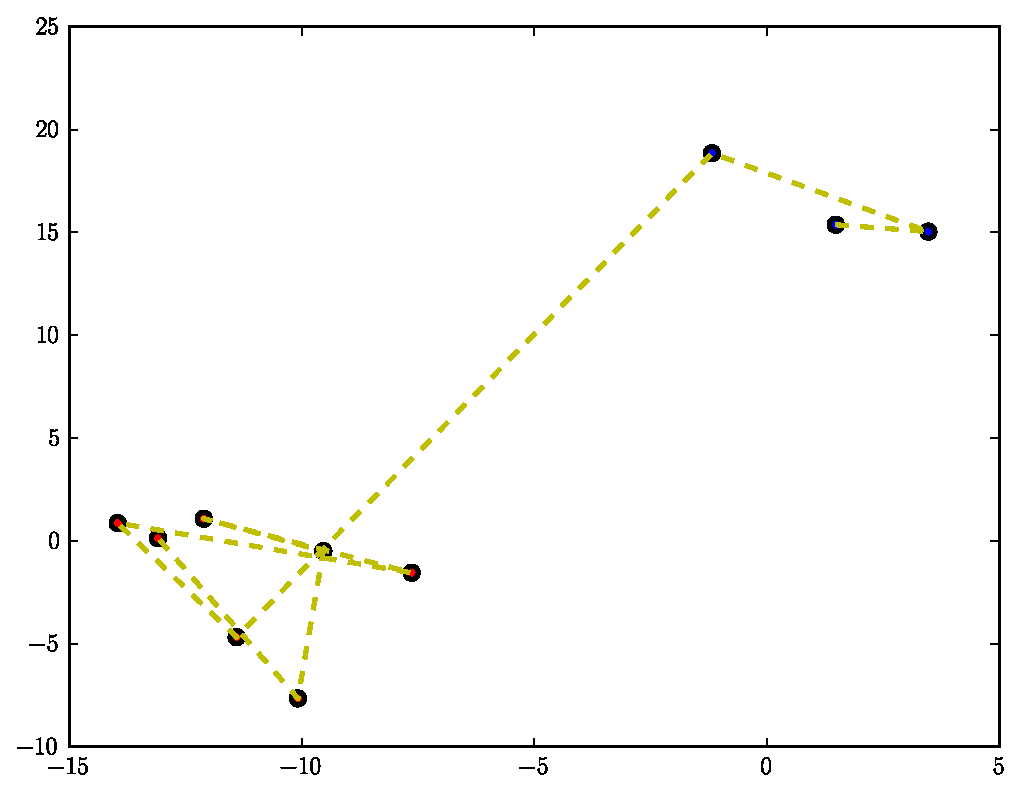
\includegraphics[width=\textwidth]{samples}
\caption{An observation sequence generated from a GMMHMM with two mixture components and two states.
The observations (points in the plane) are shown as solid dots, the color indicating from which
state they were generated. The connecting dotted lines indicate the sequential order of the observations.}
\label{fig:samples}
\end{figure}

\begin{problem}
Write a function which accepts a GMMHMM in the format above as well as an integer $T$, and which simulates the GMMHMM process, generating $T$ different observations.
Do so by implementing the following function declaration.
\begin{lstlisting}
def sample_gmmhmm(gmmhmm, T):
    """
    Simulate sampling from a GMMHMM.

    Returns
    -------
    states : ndarray of shape (T,)
        The sequence of states
    obs : ndarray of shape (T, M)
        The generated observations
    """
    pass
\end{lstlisting}

Test your function by running it on the gmmhmm given in the example, with $T=900$.
Use \li{sklearn.decomposition.PCA} with 2 components to plot the observations in two-dimensional space. 
Color the observations by state. How many clusters do you see?
\end{problem}
\newpage

The classic problems for which we normally use discrete observation HMMs can also be solved by using CDHMMs, though with continuous observations it is much more difficult to keep things numerically stable.
We will not have you implement any of the three problems for CDHMMs yourself; instead, you will use a stable module we will provide for you.
Note, however, that the techniques for solving these problems are still based on the forward-backward algorithm; the implementation may be trickier, but the mathematical
ideas are virtually the same as those for discrete HMMs.

\subsection*{Speech Recognition and Hidden Markov Models}
Hidden Markov Models are the basis of modern speech recognition systems. However, a fair amount of signal processing must precede the HMM stage, and there are other
components of speech recognition, such as language models, that we will not address in this lab.

The basic signal processing and HMM stages of the speech recognition system that we develop in this lab can be summarized as follows:
The audio to be processed is divided into small frames of approximately $30$ ms. These are short enough that we can treat the signal as being constant over these inervals. We can then take this framed signal and, through a series of transformations, represent it by mel-frequency cepstral coefficients (MFCCs), keeping only the first $M$ (say $M = 10$). Viewing these MFCCs as continuous observations in $\mathbb{R}^{M}$, we can train a GMMHMM on sequences of MFCCs for a given word, spoken multiple times. Doing this for several words, we have a collection of GMMHMMs, one for each word. Given a new speech signal, after framing and decomposing it into its MFCC array, we can score the signal against each GMMHMM, returning the word whose GMMHMM scored the highest.

Industrial-grade speech recognition systems do not train a GMMHMM for each word in a vocabulary (that would be ludicrous for a large vocabulary), but rather on \emph{phonemes}, or distinct sounds. The English language has $44$ phonemes, yielding $44$ different GMMHMMs. As you could imagine, this greatly facilitates the problem of speech recognition.  Each and every word can be represented by some combination of these $44$ distinct sounds.  By correctly classifying a signal by its phonemes, we can determine what word was spoken. Doing so is beyond the scope of this lab, so we will simply train GMMHMMs on five words/phrases: biology, mathematics, political science, psychology, and statistics.

\begin{problem}
Samples.zip contains 30 recordings for each of the words/phrases mathematics, biology, political science, psychology, and statistics. 
Remove the files that end in 00 (eg. Biology00.wav).
These audio samples are 2 seconds in
duration, recorded at a rate of 44100 samples per second, with samples stored as 16-bit signed
integers in WAV format. 
Load the recordings into Python using $scipy.io.wavfile.read$.

Extract the MFCCs from each sample using code from the file MFCC.py.
Store the MFCCs for each word in a separate list. 
You should have five lists, each containing
30 MFCC arrays, corresponding to each of the five words under consideration. 

To load and extract, use the following code:

\begin{lstlisting}
>>> samplerate, data = wavfile.read(file) # load wavfile 
>>> model = MFCC.extract(data, show = False) # extract MFCC
\end{lstlisting}
\end{problem}

For a specific word, given enough distinct samples of that word (decomposed into MFCCs), we can train a GMMHMM.
Recall, however, that the training procedure does not always produce a very effective model, as it can get stuck in a poor local minimum. 
To combat this, we will train 10 GMMHMMs for each word (using a different random initialization of the parameters each time)
and keep the model with the highest log-likelihood.

For training, we will use the python package called {\tt hmmlearn}, as this is a stable implementation of GMMHMM algorithms.
To facilitate random restarts, we need a function to provide initializations for the initial state distribution and the transition matrix.

Let \li{data} be a list of arrays, where each array is the output of the MFCC extraction for a speech sample.
Using a function \li{initialize()} that returns a random initial state distribution and row-stochastic transition matrix, we can train a GMMHMM with $5$ states
and $3$ mixture components and view its score as follows:
\begin{lstlisting}
>>> import numpy as np # Import packages 
>>> from hmmlearn import hmm
>>> startprob, transmat = initialize(5) # Get probabilities and transition matrices 
>>> model = hmm.GMMHMM(n_components=5, covariance_type="diag", init_params = "mc") # Initialize model
>>> model.startprob_ = startprob # Set probabilities and transition matrices 
>>> model.transmat_ = transmat
>>> data = train_samples[word] # Reshape data for hmmlearns fit method
>>> lengths = [data[0].shape[0]] * len(data)
>>> data_collected = np.vstack(data)
>>> model.fit(data_collected) # Fit the model
>>> model.monitor_.history[-1] # Check the score
\end{lstlisting}

%>>> import gmmhmm as hmm
%>>> startprob, transmat = initialize(5)
%>>> model = hmm.GMMHMM(n_components=5, n_mix=3, transmat=transmat, startprob=startprob, cvtype='diag')
%>>> # these values for covars_prior and var should work well for this problem
%>>> model.covars_prior = 0.01
%>>> model.fit(samples, init_params='mc', var=0.1)
%>>> print(model.logprob)

\begin{warn}
The process for problem 3 could take up to a couple of hours. 
Since you will not want to run this
more than once, you may want to save the best model for each word to disk using the pickle
module so you can use it later.
\begin{lstlisting}
>>> import pickle
>>> temp = {word: best_model}
>>> with open(word, "wb") as out:
...    pickle.dump(temp, out)
\end{lstlisting}
\end{warn}

\begin{problem}
Partition each list of MFCCs into a training set of 20 samples, and a test set of
the remaining 10 samples.
Using the training sets, train a GMMHMM on each of the words from the previous problem
with at least 10 random restarts (reinitializing and creating a new model).
Use $n\_components=5$ and $initialize(5)$.  
Keep the best model for each word (the one with the highest
log-likelihood). 
\end{problem}

Given a trained model, we would like to compute the score of a new sample.
Letting \li{obs} be an array of MFCCs for a speech sample we do this as follows:
\begin{lstlisting}
>>> score = model.score(obs)
\end{lstlisting}
We classify a new speech sample by scoring it against each of the 5 trained GMMHMMs, and returning the word corresponding to the GMMHMM with the highest score.


\begin{problem}
Classify the 10 test samples for each word. 

How does your system perform? Which words are the hardest to correctly classify?
Make a dictionary containing the accuracy of the classification of your five testing sets. 
Specifically, the words/phrases will be the keys, and the values will be the percent accuracy. 
For example, to find the accuracy for the biology model score (\li{model.score(sample)}) each model on all 10 samples in the biology test set. 
The predicted class for each sample is the class of the model with the highest score.
The accuracy of the biology model is the number of words in the biology test set that the biology model gave the highest score for over ten, since there were 10 words in the test set.
\end{problem}
























\begin{comment}

Hidden Markov Models are the basis of modern speech recognition systems. We assume that a short speech signal can be viewed as a stationary signal, and so we can divide a speech signal into small frames (approximately $30$ ms or so). We can take this framed signal and through a series of transformations represent it by mel-frequency cepstral coefficients (MFCCs), keeping only the first $K$ (say $K = 10$). Viewing these MFCCs as continuous observations in $\mathbb{R}^{K}$, we can train a GMMHMM on sequences of MFCCs for a given word, spoken multiple times. Doing this for several words, we have a collection of GMMHMMs, one for each word. Given a new speech signal, after framing and decomposing it into its MFCC array, we can score the signal against each GMMHMM, returning the word whose GMMHMM scored the highest.

In practice, a GMMHMM is not trained for each word in a vocabulary (that would be ludicrous for a large vocabulary), but rather on \emph{phonemes}, or distinct sounds. The English language has $44$ phonemes, yielding $44$ different GMMHMMs. By correctly classifying a signal by its phonemes, we can determine what word was spoken. Doing so is beyond the scope of this program, so we will simply train GMMHMMs on five words/phrases: biology, mathematics, political science, psychology, and statistics.

In a Linux environment, plug in your USB microphone headset and in the command line, enter
\texttt{arecord -l}
Note under which card the USB audio device is listed, as well as the device number. This will likely be card 1, device 0.

To record audio from the command line and save it as \texttt{test.wav} in your current working directory, enter
\texttt{arecord -f S16\_LE --rate=44100 -D hw:1,0 -d 2 test.wav}
This will record the audio from your USB microphone for $2$ seconds, sampling at a rate of $44100$ samples per second, saving the samples as signed $16$-bit numbers at the file name \texttt{test.wav}. We can read the wav file into python with the \li{scipy.io.wavfile} module:
\begin{lstlisting}
>>> import numpy as np
>>> import scipy.io.wavfile as wavfile
>>> sample = wavfile.read("test.wav")[1]
\end{lstlisting}

The object \li{sample} will be a vector of integers of length $88200 = 44100*2$. This in and of itself is not very useful. We must transform the data in a series of steps before it will be useful. We must first break the sample into \emph{frames}, each of some small length ($30$ ms). We will overlap these frames to smooth out these cutoff areas. In short, each frame will overlap with the previous by $20$ ms. Doing so with a $2$ second sample yields $198$ frames, each frame containing $1323$ values from the original sample, overlapping $882$ values with each sample immediately preceding and following it. We let $f_{n}$ denote the $n^{\text{th}}$ entry of the frame $f$.

Because we have overlapped the samples, the most significant part of a frame is the middle $441$ entries. We decrease the effects of the edges of the frame by applying a window function, making the edges nearly zero, while keeping the middle large. We use the Hamming window, defined as
\begin{equation*}
w(n) = 0.54 - 0.46 \cos \left( \frac{2\pi (n + 0.5)}{N} \right)
\end{equation*}
where $N = 1323$ is the length of the frame. We window each frame, computing $\tilde{f}_{n} = f_{n}w(n)$.

After windowing each frame, we then apply a filtering process known as \emph{preemphasis} used to improve the signal-to-noise ratio as follows:
\begin{equation*}
\widehat{f}_{n} = \tilde{f}_{n} - 0.95 \tilde{f}_{n-1}
\end{equation*}

We must next perform the discrete fourier transform of each frame, though to get a more refined view of the frequency spectrum, we must pad our vector with zeros to make it of length $2048$. We also will only keep approximately half of the returned vector, then take the square of the magnitude of each complex component.

We will ultimately be taking the logarithm of this transformed frame, so we must make sure all entries are slightly positive. We must then transform this into the \emph{mel scale}, which is a scale of pitches which listeners tend to judge to be of equal distance from one another. We make this transformation by binning the frames into $40$ bins, according to the overlapping triangular binning scheme in Figure \ref{fig:binning}.

\begin{figure}
\centering
\includegraphics[width=\textwidth]{melfilterbank.jpeg}
\caption{Binning scheme to transform linearly spaced frequency to mel scale.}
\label{fig:binning}
\end{figure}

If we want $40$ bins where the length of our padded frames is $2048$, then we can compute a \emph{mel filter bank} $M$ which is a matrix used to bin our transformed frame into the mel scale. We can now bin our frame by multiplying this matrix against the transformed frame. We also take the logarithm of the binned values, after which we compute the discrete cosine transform (DCT) of the returned values via a DCT transformation matrix, and then finally truncate to only keep ten values, called the mel frequency cepstral coefficients (MFCC). Note that we do not typically keep the first MFCC.

Normally we do this for all desired frames, storing each vector of MFCCs as a row in an array, after which we normalize by subtracting the mean of the MFCC rows, and divide by the standard deviations. We have provided you with code that allows you to compute these MFCCs quickly:
\begin{lstlisting}
>>> import MFCC
>>> mfccs = MFCC.extract(sample)
\end{lstlisting}

\begin{problem}
Record the word \emph{mathematics} as a $2$ second WAV file $20$ times, and decompose each file into its MFCC array, storing these in a list. Do this also for the words/phrases \emph{biology}, \emph{political science}, \emph{psychology}, and \emph{statistics}. Be sure you complete each word/phrase in the $2$ second window.
\end{problem}

For a specific word, given enough samples of that word decomposed into its MFCCs, we can train a GMMHMM. For this, we will use the file \li{gmmhmm.py} provided, as this is a stable implementation of GMMHMM algorithms. To facilitate random restarts, we need a function to provide initializations for the initial state distribution and the transition matrix.

\begin{problem}
Write a function that initializes the initial state distribution and transition matrix for a GMMHMM with $n$ states. You may have done this in a previous lab, so feel free to copy and paste.
\end{problem}

Let \li{samples} be a list of arrays, where each row in each array is a set of MFCCs corresponding to a frame in a sample for a given word. Using a function \li{initialize()} that returns a random initial state distribution and transition matrix, we will show how to train a GMMHMM with $5$ states, each having an output distribution as a GMM with $3$ mixture components. We also look at the log-likelihood of the data, given the trained model.
\begin{lstlisting}
>>> import gmmhmm as hmm
>>> startprob, transmat = initialize(5)
>>> model = hmm.GMMHMM(n_components=5, n_mix=3, transmat=transmat, startprob=startprob, cvtype='diag')
>>> model.covars_prior = 0.01
>>> model.fit(samples, init_params='mc', var=0.1)
>>> print(model.logprob)
\end{lstlisting}

\begin{problem}
Train a GMMHMM on each of the words you previously recorded with at least $10$ random restarts, keeping the best model for each word. You might want to do this in parallel to save time.
\end{problem}

Given a trained model, we would like to compute the log-likelihood of a new sample. Letting \li{obs} be an array, each row of which is a set of MFCCs for a frame in a sample, we do this as follows:
\begin{lstlisting}
>>> score = model.score(obs)
\end{lstlisting}

\begin{problem}
Write a function that records a sample, converts it into its MFCC array, and then scores it on each of the five trained models. Return the word corresponding to the highest scoring model. Test your speech recognition system on each of the five words multiple times. How does it perform?
\end{problem}
\end{comment} 
